
The probabilities from the data set are in the following figure.


\begin{center}
    Table of results
    \begin{tabular}{ |c|c| } 
      
     \hline
     Method & Accuracy \\ 
     Random & 33.3\% \\ 
     Threshold Sum & 39.2\% \\ 
     Threshold Sum and Square & 32.7\% \\
     Single-Axis Guassian & 38.5\% \\
     FFT distance & 47.5\% \\
     \hline
     
    \end{tabular}
\end{center}



\begin{center}    
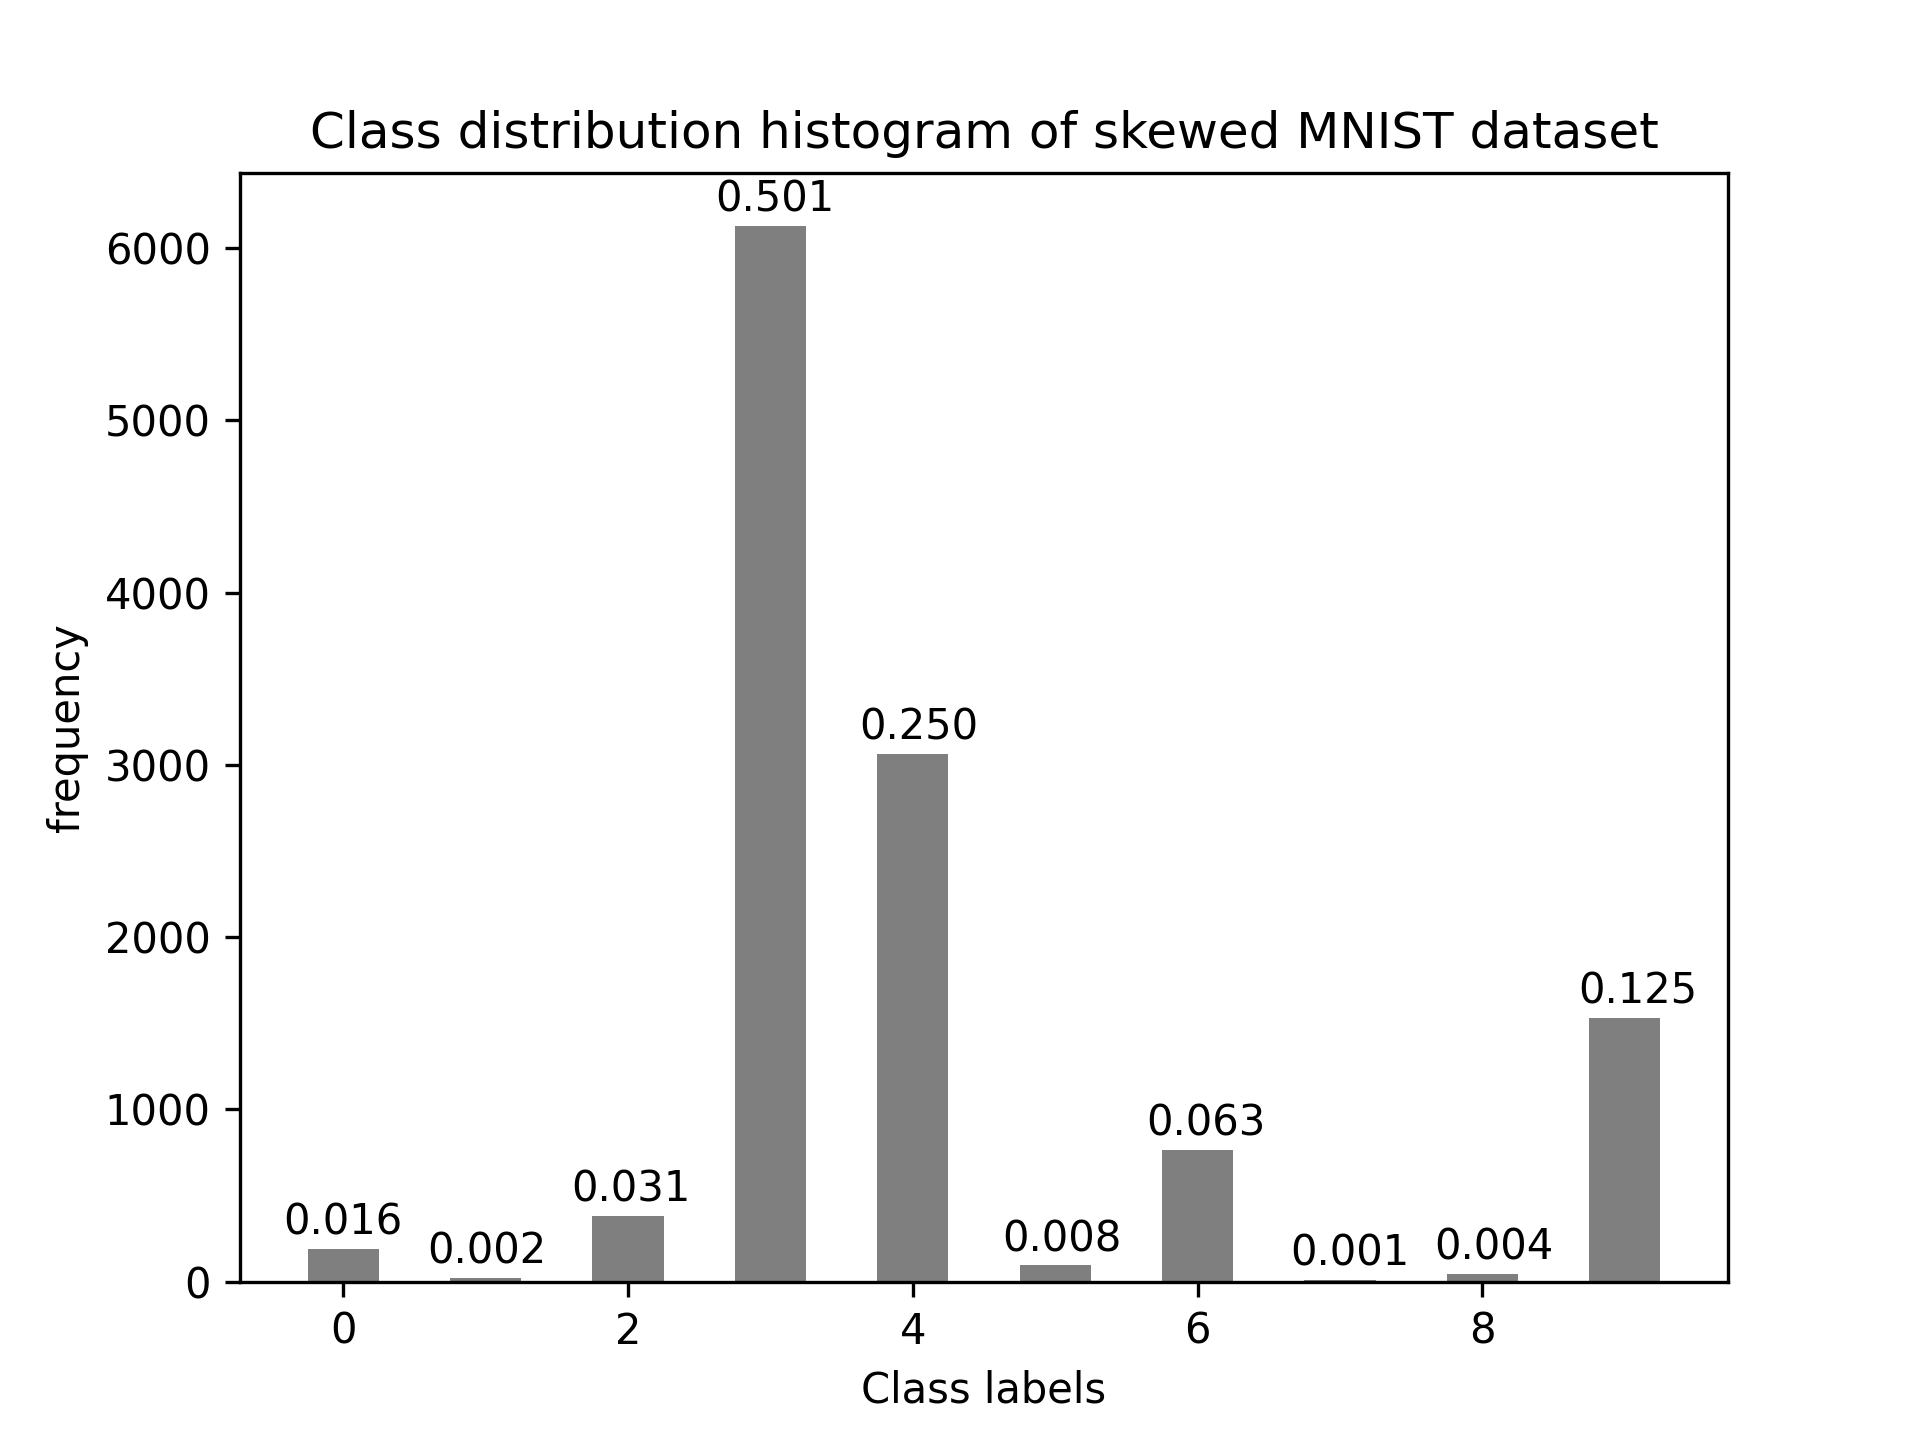
\includegraphics[width=0.5\textwidth]{class_histogram.png}
\captionof{figure}{Histogram of True Classes}
\end{center}  


\begin{center}
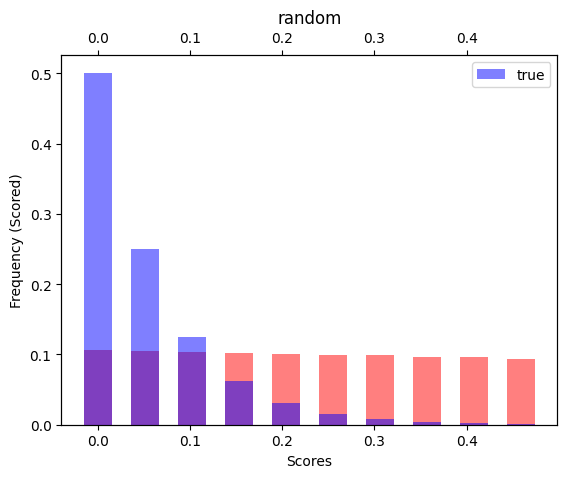
\includegraphics[width=0.35\textwidth]{random_pareto.png}
\captionof{figure}{Sorted histogram of random method scores}
\end{center}
    

\begin{center}
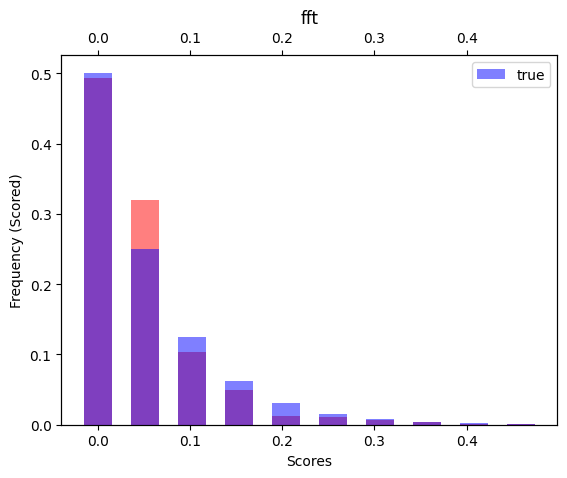
\includegraphics[width=0.35\textwidth]{fft_pareto.png}
\captionof{figure}{Sorted histogram of FFT method scores}
\end{center}
    

